
\chapter{\gls{BNP} inference within \glspl{PPL}} \label{BNP_PPL}
In this chapter we focus on the task of performing inference within a \gls{PPL} for models with an infinite dimensional component, also called \gls{BNP} models.
For now we have restricted ourselves to infinite mixture models, but we hope that our framework will enable efficient sampling for other \gls{BNP} models such as the infinite \acrlong{HMM} \cite{Beal02theinfinite}. We have also focused our study on sampling methods, but \acrlong{VI} is considered in Section \ref{BNP_VI}.

\section{Recursion is key} \label{recursion}

In \glspl{PPL}, to transform a variable in a random variable, one only needed to write \texttt{x = sample(Dist(parameters))}. Then the posterior distribution (given some observations) of \texttt{x} will automatically be performed during the inference scheme.
The Bayesian setting thus naturally fits the framework of \glspl{PPL}.
Yet, we believe that there is more  than just a connection between Bayesian inference and \glspl{PPL}, but that there is also a connection between \acrlong{BNP} and High-order \gls{PPL}.

Working with \gls{BNP} models can be impossible because of the constraints of computers.
A \gls{NRM} $P$ can be written \cite{Kingman:1967kn} as
$$P = \sum_{k \ge 1}{\tilde{p}_k \delta_{X^\star_k}} $$
where $\left(\tilde{p}_k, X^\star_k \right)_{k \ge 1}$ is an infinite collection of weights and atoms.
Discrete probability measures with countable support such as \acrlongpl{NRM} cannot be represented in a computer in a naïve manner since a machine has finite memory.
Other representations of such objects must be used, if one hope to denote them in a program.

One key notion in programming languages which will be crucial is the concept of \textit{lazy evaluation} (or \textit{laziness}). It is an evaluation strategy which delays the evaluation of an expression until its value is needed and which also avoids repeated evaluations.
Lazy evaluation is often combined with \textit{memoization}, as described in \cite{Bentley:1982:WEP:539147}. After a function's value is computed for that parameter or set of parameters, the result is stored in a lookup table that is indexed by the values of those parameters; the next time the function is called, the table is consulted to determine whether the result for that combination of parameter values is already available. If so, the stored result is simply returned. If not, the function is evaluated and another entry is added to the lookup table for reuse.

Instead of hoping to construct the entire infinite sequence $\left({p}_k, X^\star_k \right)_{k \ge 1}$, we will only ``lazily'' sample $\left({p}_k, X^\star_k \right)$, i.e. when we need them.
Since we work with homogeneous \glspl{CRM}, the $\{X^\star_k\}_{k \ge 1}$ are independent and identically distributed according to the base distribution. Sampling the $(X^\star_k)_{k \ge 1}$ as we need them is therefore trivial. Yet, how could we lazily sample the $({p}_k)_{k \ge 1}$ ?
In Subsection \ref{DP}, we presented the stick-breaking process, a generative process for constructing of a size-biased permutation of $({p}_k)_{k \ge 1}$, denoted $(\tilde{p}_k)_{k \ge 1}$.
In Section \ref{SBS} we explore other generative processes, for more generic \gls{BNP} classes. For now, Let us recall the construction given by \cite{sethuraman94} for the stick-breaking process:


\begin{gather*}
V_1 \sim \text{Beta}(1, \alpha) \\
V_2 \sim \text{Beta}(1, \alpha) \\
\vdots \\
V_j \sim \text{Beta}(1, \alpha) \\
\vdots \\
\tilde{p}_k = V_k \prod_{j=1}^{k-1}(1-V_j) \ \ k= 1,2,\dots
\end{gather*}

Therefore, $\tilde{p}_k$ can be seen as the probability of the following sequence of outcomes: $k-1$ Bernouilli draws with respective probabilities $V_j \ , j=1,\dots,k-1$, all yield failure, and one last Bernouilli draw with probability $V_k$ yields success.
How can this be interpreted as a generative process on an infinite set of discrete outcomes ?
%With this insight so as to sample from a \gls{CRP}, or equivalently from a \gls{DP} with a base distribution on the natural numbers.
Imagine ``walking'' down the natural numbers in order, flipping a coin with weight $V_k$ (also called stick) for each one; if the coin comes up \texttt{false}, we continue to the next natural number; if the coin comes up \texttt{true}, we stop and return the current natural number. The probability of getting the natural number $k$ is given by $\tilde{p}_k$ defined above. This is formalised by the procedure \texttt{pickStick} in the code sample \ref{code:DP_SB} below.

\begin{lstlisting}[caption={\acrlong{DP} stick-breaking representation written in Julia.},captionpos=b,label=code:DP_SB]
function pickStick(sticks, J) = begin
  return rand(Bernouilli(sticks(J))) ? J : pickStick(sticks, J+1)
end

function makeSticks($\alpha$) =  begin
  sticks = @memoize (index) -> rand(Beta(1, $\alpha$))
  return () -> pickStick(sticks, 1)
end
\end{lstlisting}

The individual $V_k$ are drawn lazily, only generating new ones when we have walked out further than furthest previous time. This is the role of the procedure \texttt{makeSticks} which uses memoization to enforce this property. Even though we started by imagining an infinite set of sticks we only ever construct a finite subset of them. The above construction of the \gls{DP} defines a distribution over the infinite set of natural numbers.

Remark that the function \texttt{pickStick} is written in a special fashion: it is built via a \textit{recursion}. A \textit{recursive} function has one or more base cases for which the function produces a result trivially (without recurring), and one or more recursive cases for which the program recurs (calls itself). For programming languages, allowing recursion means allowing a function to call itself within the program text. Moreover, before calling \texttt{pickStick}, no one knows the integer which will be returned, i.e. the number of recursion calls, since it is a random variable by construction.

Recall that high-order \glspl{PPL} allow complex control flow, including stochastic recursion (stated in Section \ref{PPL_history}). \textit{Stochastic} or \textit{unbounded} recursion simply means that the number of recursive calls (also called \textit{depth} of the recursion) is random or unbounded. Therefore, the \gls{DP} stick-breaking process can be written and executed with such high-order \glspl{PPL}.

\glspl{PPL} are some sort of \textit{simulators}, models need to be written as generative processes. Executing such a model -- as is -- via a \gls{PPL}'s interpreter, is sampling from its prior distribution. Once one can write a model as a generative process, (i.e can sample from the model's prior), the \gls{PPL} can perform inference on the latent variables. Consequently, for \gls{BNP} models, a representation similar to the stick-breaking process for the \gls{DP}, seems to be necessary.


\subsection{Implementation details}
As highlighted, recursion is key to denote \gls{BNP} models in a \gls{PPL}.
A function is called \textit{tail-recursive} when the recursive call happens as the final action in a function (as for \texttt{pickStick}), in which case it can happen without the function call stack growing. In \gls{CPS}, there is no stack -- all function calls are tail calls, hence all recursive functions are tail-recursive.

Clojure provides special forms \emph{loop} and \emph{recur} for writing tail-recursive programs. Anglican programs are \gls{CPS}-converted and do not use the stack. Therefore recursive calls in the Anglican \gls{PPL} cannot lead to stack overflow.
Without such a specific \emph{recur} operator, the call stack can exceed its maximum size and yields errors.

\subsection{Existing work}

Most high-order \glspl{PPL} indeed already handle some \gls{BNP} models \cite{Goodman:2012uq,wood-aistats-2014,probmods2}.
See \footnote{\url{http://www.robots.ox.ac.uk/~fwood/anglican/examples/index.html}} for Anglican's examples of Hierarchical Dirichlet Process or Probabilistic Deterministic Infinite Automata. See also \footnote{\url{https://probmods.org/chapters/12-non-parametric-models.html}} for WebPPL's example of Infinite Hidden Markov Models or Infinite Relational Model.
Yet, their experiments are mostly limited to \acrlong{DP}, \acrlong{PY} or hierarchical versions of these processes, and often focused on sampling from priors. When performing inference,
the used scheme is usually a particle algorithm such as \acrlong{SMC} or \acrlong{PG}.


\section{Generative constructions of random probability measures} \label{SBS}
Previously, we recalled that to be able to denote a model in a \gls{PPL}, one should know how to sample from its prior, i.e. know a generative construction.
We also highlighted the fact that such generative processes are implemented via stochastic recursion.

\subsection{Stick-breaking processes} \label{stick-breaking}

The first comprehensive treatment of stick-breaking priors dates back to the paper by Ishwaran and James \cite{Ishwaran:2001dw}. There, they introduced a class of stick-breaking priors including as special cases the \acrlong{DP} by Ferguson \cite{ferguson73} and the two parameter Poisson-Dirichlet process by Perman et al. \cite{Perman:1992ke}. Specifically, let $H_0$ be a nonatomic probability measure on a complete and separable metric space $\mathbb{X}$.
% equipped with the Borel σ-field X .
Also, let $(V_i)_{i \ge 1}$ be a sequence of independent random variables such that $\sum_{i \ge 1}{\mathbb{E}[\log(1 - V_i)]} = - \infty$.
Based on such $V_i$'s, they define a sequence of random probabilities $(\tilde{p}_k)_{k \ge 1}$ as $\tilde{p}_1 = V_1$ and
\begin{equation} \label{eq:Stick_breaking}
\tilde{p}_k = V_k \prod_{j=1}^{k-1}{(1-V_j)} 
\end{equation}
for each $k > 1$, and let $(X^\star_k)_{k \ge 1}$ be a sequence of random variables, independent
of $(\tilde{p}_k)_{k \ge 1}$, and independent and identically distributed according to $H_0$. Then,
$$ P = \sum_{k \ge 1}{\tilde{p}_k \delta_{X_k^\star}} $$
is a stick-breaking prior in the class of Ishwaran and James \cite{Ishwaran:2001dw}.

For any $\sigma \in [0,1)$ and $\theta > -\sigma$, the stick-breaking representation of the two parameter Poisson-Dirichlet process is recovered by assuming the $V_k$'s to be distributed according to the Beta distribution with parameter $(1 - \sigma, \theta + k\sigma)$ for each $k \ge 1$.
The stick-breaking representation of the \gls{DP}, which was first derived by Sethuraman \cite{sethuraman94}, is also recovered as special case, by setting $\sigma = 0$.

Apart from the two parameter Poisson-Dirichlet process, most of the discrete random probability measures do not admit a stick-breaking representation in terms of a collection of independent $V_i$'s.%, but in terms of conditional distributions of $Z_k$'s given $(Z_1,\dots,Z_{k-1})$.

As an example, Favaro et al. \cite{Favaro:2012ht} derived the stick-breaking representation of the normalized inverse Gaussian process introduced in Lijoi et al. \cite{Lijoi:2005ku}. Specifically, let $b > 0$ and let $(V_k)_{k \ge 1}$ be a sequence of dependent random variables such that, for each $k \ge 1$, the conditional distribution of $V_k$ given $(V_1,\dots,V_{k-1})$ coincides with the distribution of the random variable
\begin{equation} \label{eq:IGP}
\frac{X_k}{X_k + Y_k}
\end{equation}
where $X_k$ is distributed according to the generalized inverse Gaussian distribution and $Y_k$ is distributed according to the positive $\frac{1}{2}$-stable distribution.

According to Favaro et al \cite{Favaro:2014bo}, the normalized inverse Gaussian process \cite{Favaro:2012ht} is the first example of a prior admitting a stick-breaking representation in terms of dependent  $V_k$'s, and such that for any $k \ge 1$ the conditional distribution of $V_k$ given $(V_1,\dots,V_{k-1})$ is characterized by means of a straightforward transformation of random variables as in \ref{eq:IGP}.
Favaro et al \cite{Favaro:2014bo} construct a similar transformation to build a stick-breaking process for a subclass of $\sigma$-stable Poisson-Kingman processes.

Similarly, James \cite{James:2013uk} builds a stick-breaking process for the class of $\text{PG}(\alpha,\zeta)$-Generalized Gamma Processes. The $V_k$'s can be generated via the following construction:
\begin{gather*}
\zeta_0 \sim \zeta \\
\vdots \\
\zeta_k = \zeta_0 + \sum_{j=1}^{k-1}{e_j},\ e_j \sim \text{Exp}(1) \\
R_k = \left(\frac{\zeta_{k-1}}{\zeta_k}\right)^{1/\alpha} \\
V_k = 1 - \beta_k(1 - R_k), \ \beta_k \sim \text{Beta}(1-\alpha,\alpha) \\
\vdots \\
\tilde{p}_k = V_k \prod_{j=1}^{k-1}(1-V_j) \ \ ,k= 1,2,\dots
\end{gather*}

Since the size-biased sequence of weights $(\tilde{p}_k)_{k \ge 1}$ is defined through Equation \ref{eq:Stick_breaking} for stick-breaking processes, it can be generated in the same way than described in the previous Section (\ref{recursion}): drawing Bernouilli's with parameters $V_k$'s until success, then return integer $k$. Stochastic recursion is therefore the crux of the  implementation of stick-breaking processes.

\subsection{Size-biased generative processes}
% \subsection{\acrlong{PKP}}

The \gls{PKP} generative process (\acrlong{SBS}) described in Section \ref{PKP}, is reminiscent of the well known stick breaking construction from Ishwaran \& James \cite{Ishwaran:2001dw}, where a stick of length one is successively broken as in Figure \ref{fig:PY_stick_breaking}.
This \gls{SBS} process is illustrated in Figure \ref{fig:PK_generative_process} and schematically recalled below:
\begin{gather*}
T \sim \gamma \\
\tilde{J}_1|T \sim \text{SBS}(T) \\
\tilde{J}_2|T,\tilde{J}_1 \sim \text{SBS}(T - \tilde{J}_1) \\
\vdots \\
\tilde{J}_{l}|T,\tilde{J}_1,\dots,\tilde{J}_{l-1} \sim \text{SBS}(T - \sum_{i<l} \tilde{J}_i) \\
\vdots \\
\end{gather*}
\begin{figure}[h!]
  \centering
  \begin{minipage}[b]{0.48\textwidth}
    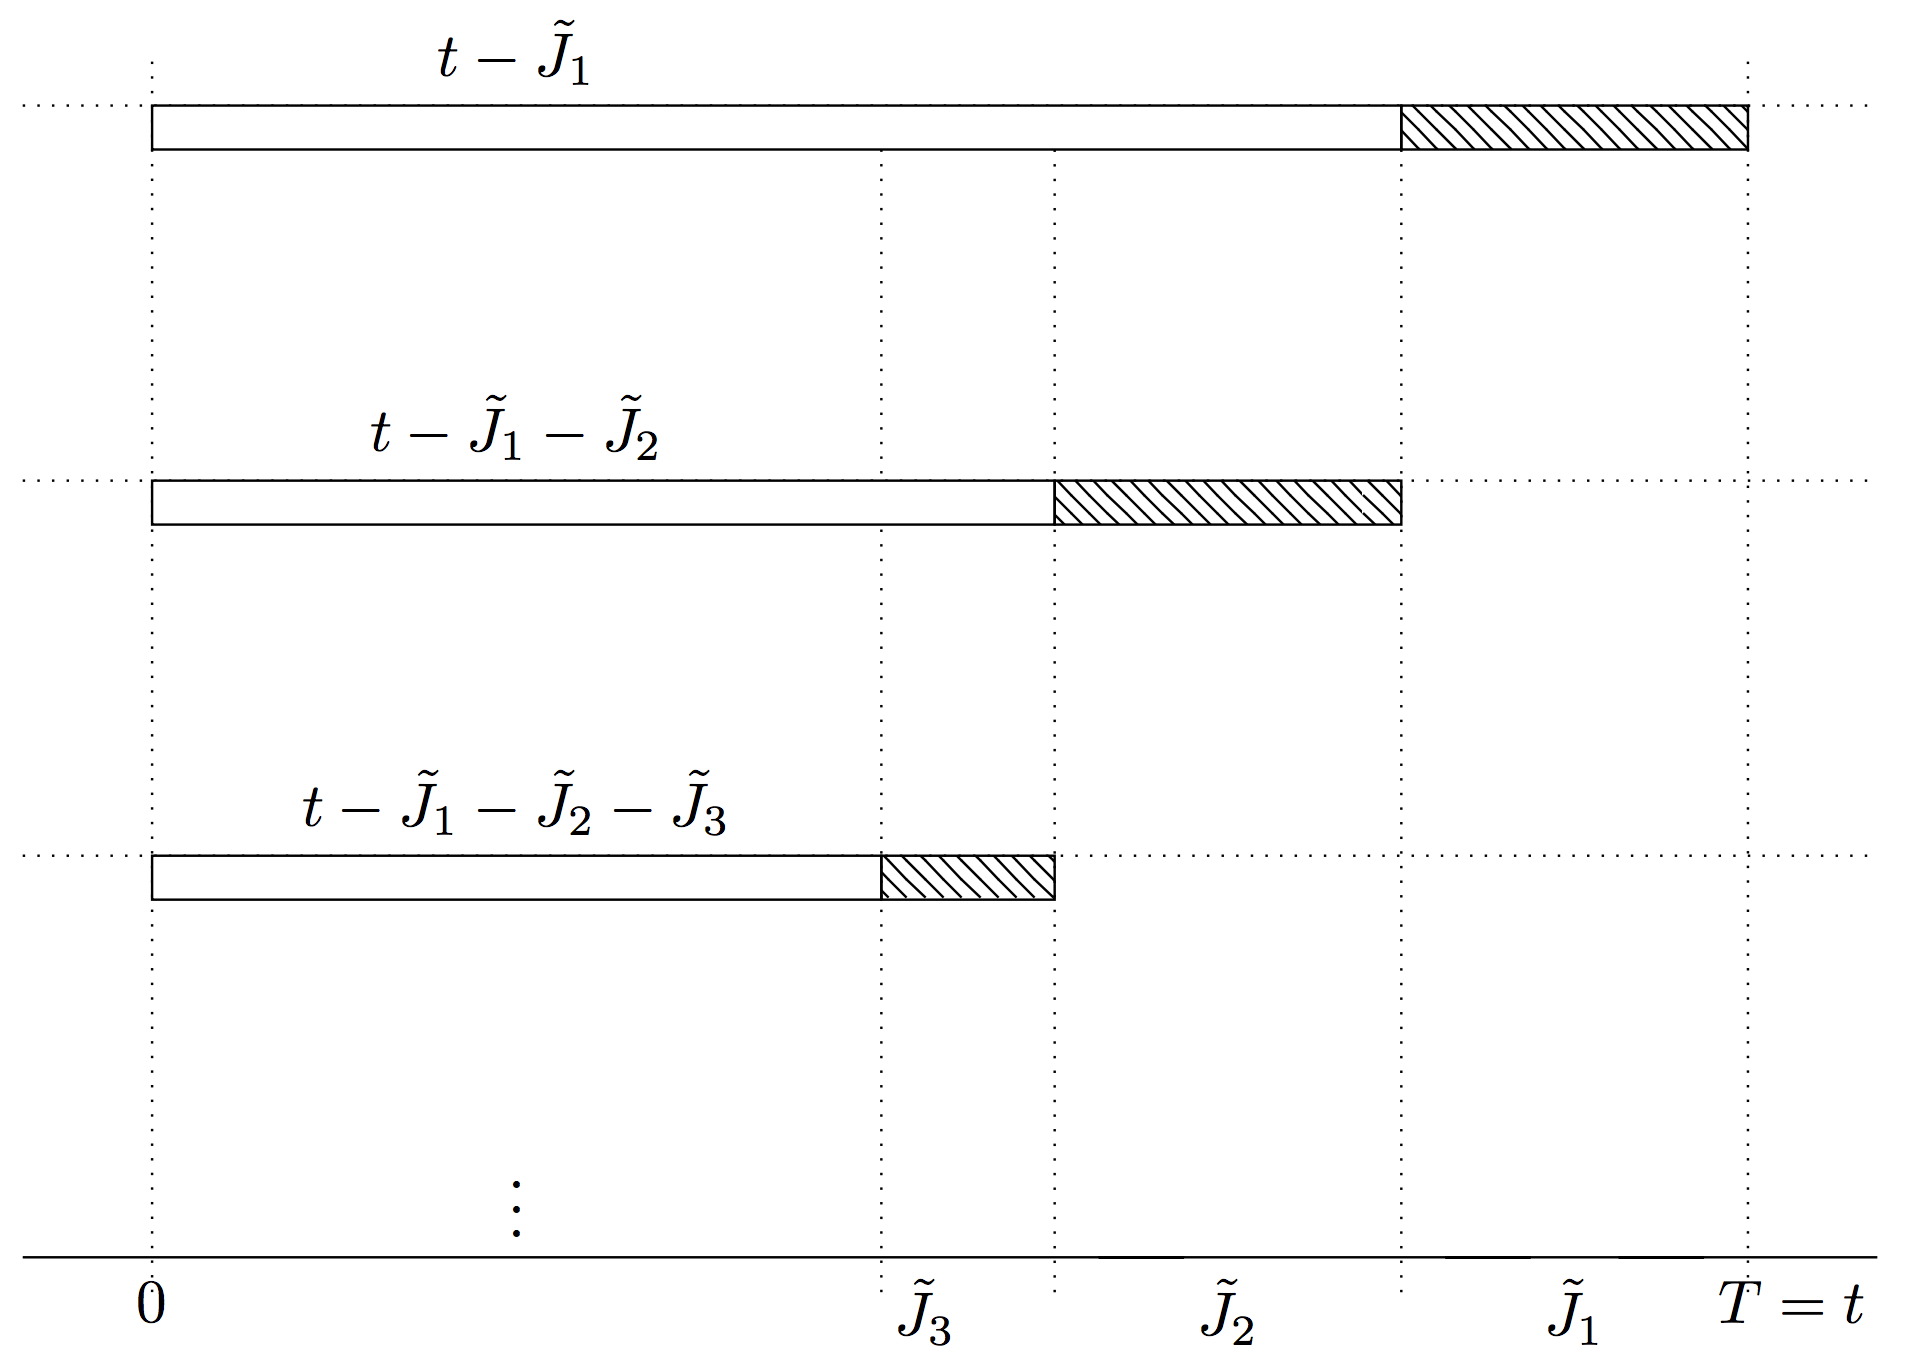
\includegraphics[width=\textwidth]{PK_generative_process2.png}
    \caption{Generative process of Poisson-Kingman Process. Source: \cite{LomeliThesis}.}
    \label{fig:PK_generative_process}
  \end{minipage}
  \hfill
  \begin{minipage}[b]{0.48\textwidth}
    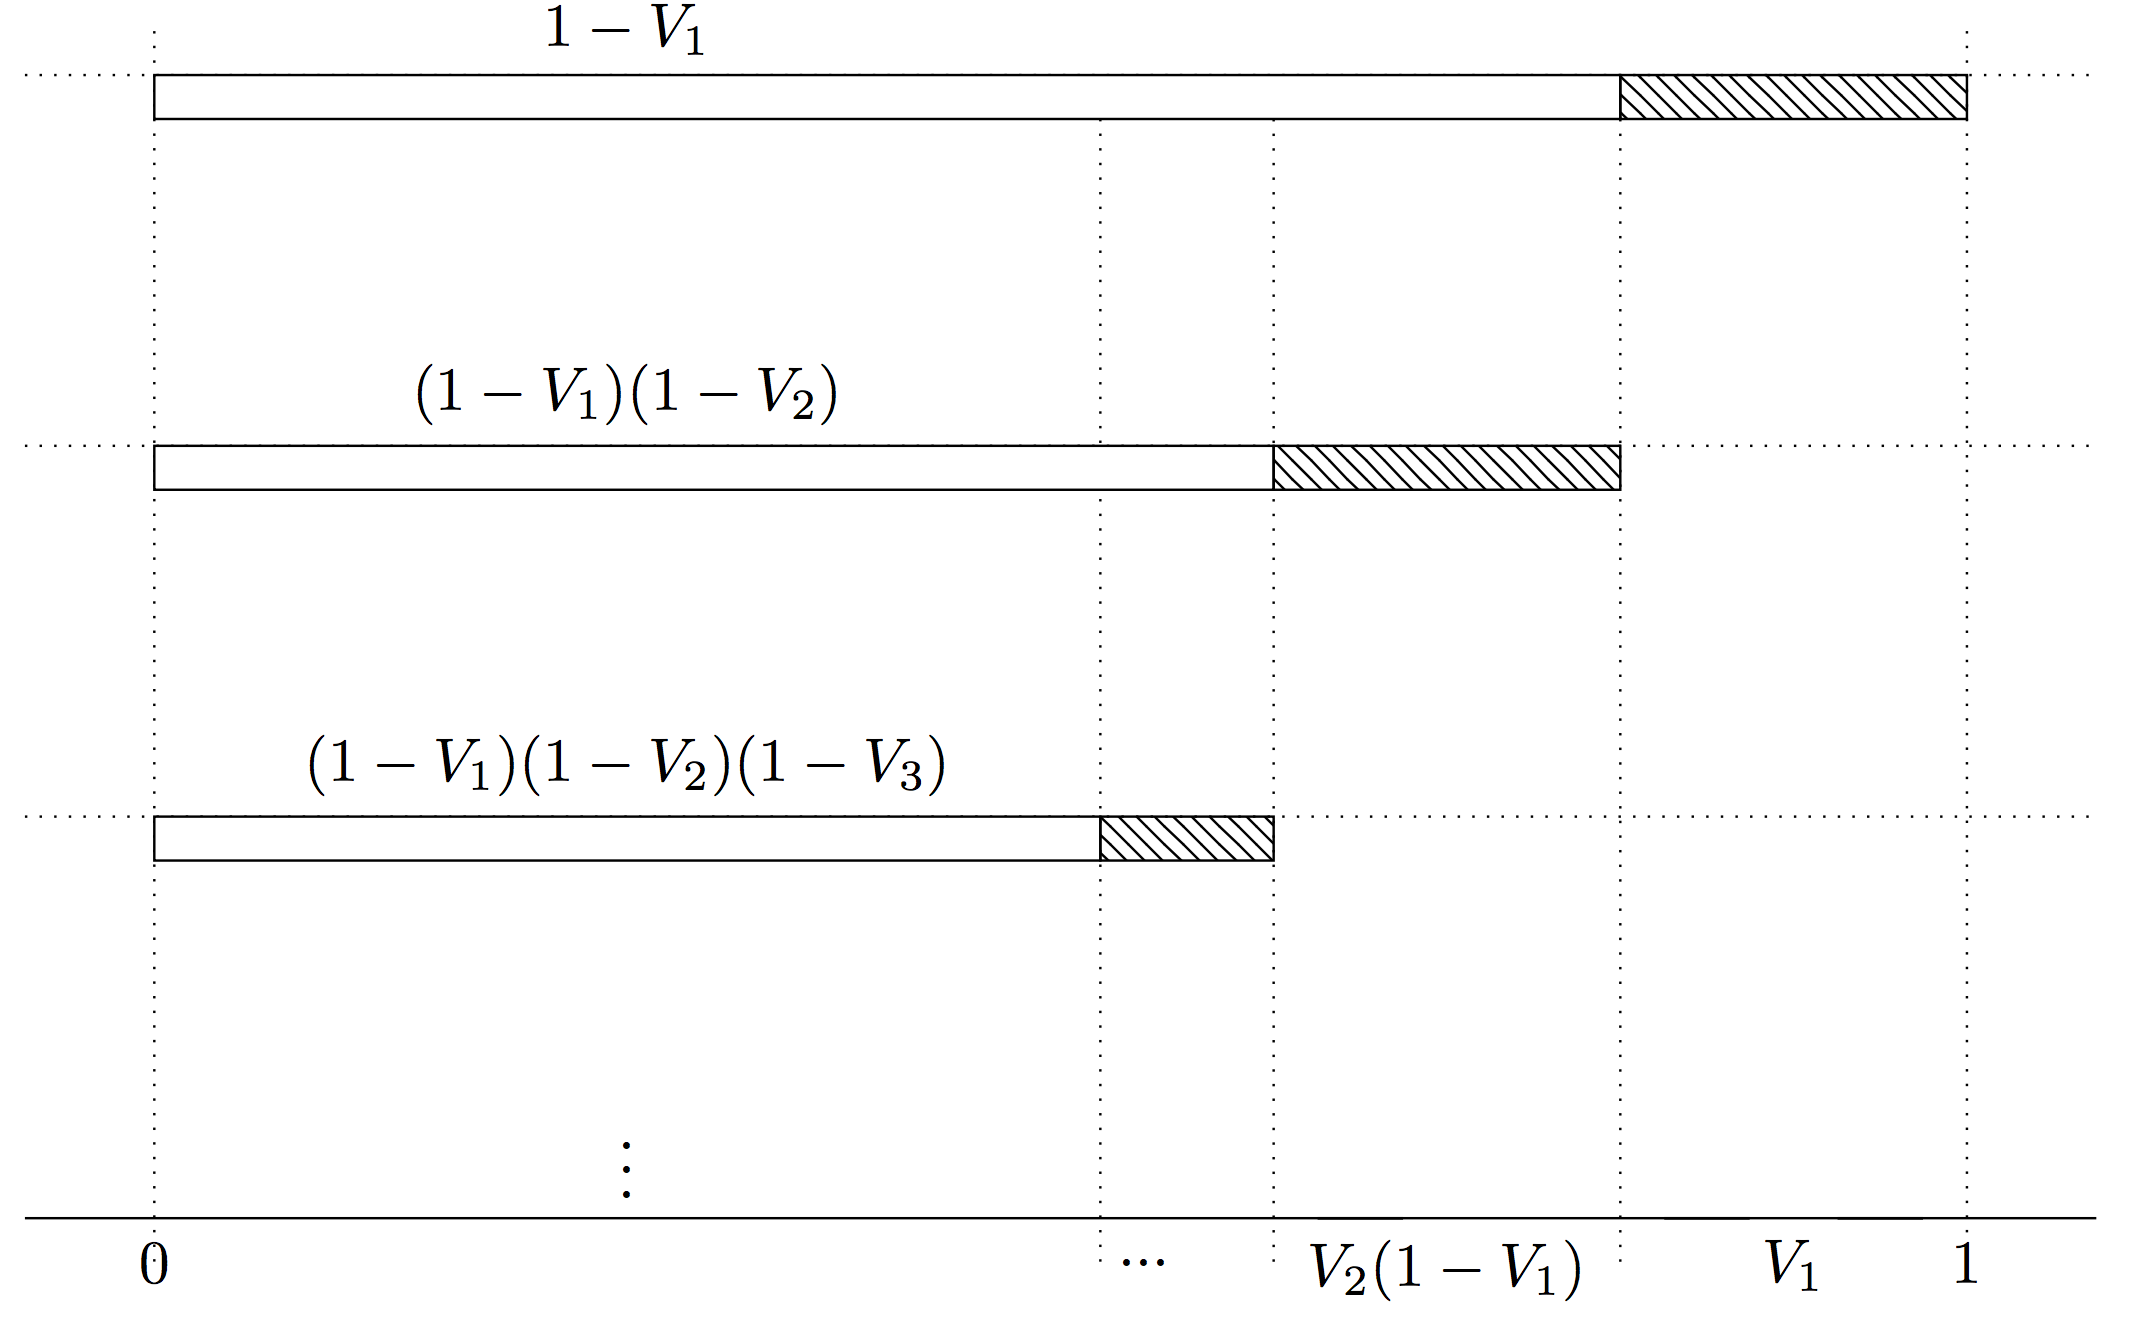
\includegraphics[width=\textwidth]{PY_stick_breaking2.png}
    \caption{Stick-breaking construction. Source: \cite{LomeliThesis}.}
    \label{fig:PY_stick_breaking}
  \end{minipage}
\end{figure}
However, by starting with Equation (\ref{eq:perman2}), one can recover the usual stick-breaking construction due to two useful identities (in distribution):
\begin{equation} \label{eq:SBS1}
\tilde{p}_k := \frac{\tilde{J}_k}{T} \ \text{for} \ k=1,\dots
\end{equation}
\begin{equation} \label{eq:SBS2}
V_k := \frac{\tilde{p}_k}{1 - \sum_{j=1}^{k-1}{\tilde{p}_j}} \ \text{for} \ k=1,\dots
\end{equation}

Indeed, equivalently to Equation (\ref{eq:SBS2}), we have $\tilde{p}_k = V_k \prod_{j=1}^{k-1}{(1-V_j)}$ for all $k \ge 1$, which is of the same form as Equation (\ref{eq:Stick_breaking}) for the usual stick-breaking process.
However, in general, the stick random variables $(V_k)_{k \ge 1}$ from Equation (\ref{eq:SBS1}), form a sequence of dependent random variables, except for some simple process as the \gls{DP} and \gls{PY}, see Pitman \cite{PitmanRDD} for details.
Similarly to stick-breaking constructions, \acrlongpl{PKP} can therefore be constructed in a generative manner and implemented via (stochastic) recursion.

%(\ref{eq:perman2})
%By reparameterizing the model using these identities and then obtain the corresponding joint in terms of $(0,1)$-valued stick-breaking weights $\{{V}_k\}_{k \ge 1}$ which correspond to the usual stick-breaking representation. This joint distribution is for a general Lévy measure $\rho$, density $f_\rho$ and it is conditioned on the valued of the random variable $T$.
%The standard Stick breaking representations can be recovered for the Dirichlet and Pitman-Yor processes, for a specific choice of $\rho$ and if we integrate out T. For instance, the \gls{PY} stick breaking representation \cite{Ishwaran:2001dw} can be recovered from the \acrlong{SBS} generative process of Section 2.5 after integrating out the total mass $T$, a change of variables and the following distribution for the total mass is substituted
%$$ \gamma_{\text{PY}}(t) = \frac{\Gamma(\theta+1)}{\Gamma(\theta / \alpha + 1)}t^{-\theta} f_\sigma(t) 1_{(0,\infty)}(t), \quad \theta > -\sigma $$
%where $f_\sigma$ is the density of a $\sigma$-Stable random variable.

\paragraph{Practical aspects of \gls{SBS}}
In the \acrlong{SBS} process (described in Section \ref{PKP}), when a random variable $X_i$ takes the value of an atom which has not yet been sampled, a new atom $X^\star_{k+1}$ must be sampled, along with its associated weight $\tilde{J}_{k+1}$. The new atom $X_{k+1}^\star$ is drawn from $H_0$, while its mass is drawn from
\begin{equation} \label{eq:SBS3}
\mathbb{P}_{\rho,H_0}(\tilde{J}_{k+1} \in ds_{k+1} | T \in dt_k) = \frac{s_{k+1}}{t_k}\rho(ds_{k+1})\frac{f_\rho(t_k - s_{k+1})}{f_\rho(t_k)}
\end{equation}

Yet, even if we know the density of the distribution of $\tilde{J}_{k}|T,\tilde{J}_1,\dots,\tilde{J}_{k-1}$, we do not necessarily know how to sample from it.
We are currently working on a generic way to sample from such as distribution. We could restrict to Lévy measures with tractable intensity -- which can be evaluated pointwise -- thus excluding $\sigma$-Stable \gls{PK}. A simple rejection sampling scheme with proposal $\mathcal{U}(0, T_k)$ might be sufficient.
Nonetheless, there are particular cases for which we already know how to sample from these distributions. Lomeli et al \cite{Lomeli:2015vd} propose a simple rejection sampling scheme with uniform proposal to tackle the $-\log$Beta \gls{PK} process. Favaro et al \cite{Favaro:2014bo} give an identity from which iid samples can be drawn for a subclass of $\sigma$-Stable \gls{PKP}.

\textcolor{red}{Sampling from -logBeta PKP: graph of the sampled random measure}

\section{Models of interest}
We focus on infinite mixture models described in Section \ref{mixture_models}.
The stick-breaking construction previously described in Section \ref{recursion} defines a distribution over the infinite set of natural numbers via the sequence of weights $(\tilde{p}_k)_{k \ge 1}$. Ultimately we would like a distribution not over the natural numbers themselves, but over an infinite set of samples from some other distribution $H_0$ (called the base distribution) which will represent our mixture components. Using the homogeneous assumption (of the underlying \gls{CRM}), we can easily generalise the \gls{DP} code that we wrote to this setting by using \texttt{@memoize} to associate to each natural number, a draw from the base distribution.
This is what the code sample (\ref{code:DP}) formalises.

\begin{lstlisting}[caption={\acrlong{DP} with base distribution $H_0$ written in Julia.},captionpos=b,label=code:DP]
function DPmem($\alpha$,$H_0$) =    begin
  augmentedProc = @memoize (stickIndex) -> rand($H_0$)
  DP = makeSticks($\alpha$)
  return () -> augmentedProc(DP())
end
\end{lstlisting}

We uses this \gls{DP} construction as a prior over mixture components so as to build an infinite mixture model (see code sample \ref{code:IMM}).

The real code of the \gls{DP} stick-breaking process and of the infinite mixture model which has been used for our experiments can be found on Github \footnote{\url{https://github.com/emilemathieu/BNPMixPPL/blob/master/src/codebase/DPMixture2.jl}}.

\begin{lstlisting}[caption={Nonconjugate infinite mixture model written in Turing.jl.},captionpos=b,label=code:IMM]
@model InfiniteMixutre(y) = begin
  N = length(y)
  $\alpha$ =  10.0
  m ~ Normal(meanMean, 1.0/sqrt(meanPrecision)) # Sample statement
  s ~ Gamma(precisionShape, 1.0/precisionInvScale) # Sample statement
  P = rand(DP($\alpha$, Normal(m, 1.0/sqrt(s)))) # Random probability measure

  x = tzeros(N)
  for i in 1:N
    x[i] ~ P # Sample statement
    y[i] ~ Normal(x[i], 1.0/sqrt(s)) # Observe statement
  end

  return x
end
\end{lstlisting}

Note the use of the \texttt{for-loop} above so as to express the model as \acrlong{SSM}. Such a formulation allow to make use of particle algorithms (described in Subsections \ref{IS} and \ref{PMCMC}) thanks to the sequence of \texttt{observe} statements.
In the code sample (\ref{code:IMM}) for the infinite mixture model, the \texttt{DP} \acrlong{RPM} can be replaced by another \acrlong{NRM} of \acrlong{PK} \gls{RPM}.


\paragraph{Stochastic memoization}
Discrete Random Probability Measures can be seen through the interesting perspective of \textit{stochastic memoization} \footnote{\url{https://probmods.org/chapters/12-non-parametric-models.html}}, which is an in-between (deterministic) memoization and no memoization.
Higher-order procedures such as \texttt{DPmem} (defined above) transform a procedure into one that sometimes reuses its returned values, and sometimes generate new values. These procedures are called \textit{stochastic memoizers} by Goodman et al. \cite{Goodman:2012uq}.
For instance with the \gls{DP}, setting $\alpha = 0$ recovers a deterministic memoization whereas setting $\alpha \rightarrow \infty$ yields no memoization at all.

\section{Sampler}
% calculus for SMC for BNP mixture with fixed parameters
% fixed parameters are not a assumption, since can be made random then with PMCMC

Now that we have detailed and implemented a generative process (i.e. sampling from the prior) for our class of models, we focus in this section on the sampling scheme to use within the \acrlong{PPL}.
As explained in Section (\ref{IS}), the \acrfull{SMC} algorithm breaks down the overall inference problem into a series of target distributions which get incrementally closer to the distribution of interest. These intermediate target distributions live in smaller spaces than the overall posterior distribution. This class of methods is consequently well suited for the high-dimensional models that we are considering.
Since, we are interested in models where hyper-parameters are also random variables (see code (\ref{code:IMM})), we focus on \acrlong{PMCMC} methods.

We started by using \acrlong{PG} (see Section (\ref{PMCMC})) targeting the cluster components and assignments with the conditional \gls{SMC} and the hyper-parameters with an \gls{HMC}.

\textcolor{red}{Posterior distribution of hyperparmeters for DP mixture with PG}
\textcolor{red}{ESS of mixture components for DP mixture, highlight path degeneracy}

Unsurprisingly we observed a big path degeneracy issue. Figure \ref{} shows that the first $X_t$'s ($t$ close to $1$) have way lower \gls{ESS} compared to $X_t$'s at the end of the sequence. This is a well-known issue, which is tackled in \gls{PGAS} and \gls{IPMCMC}.
\gls{PMMH} should bring symmetry in the \gls{ESS} graph (\gls{ESS} for the $y$-axis and $t$ index for the $x$-axis), i.e. all $X_t$'s should have in average the same \gls{ESS}.
The path degeneracy issue been tackled by the \gls{PGAS} and \gls{IPMCMC} algorithms (see Section (\ref{PMCMC}) for more details).
We believe that the \gls{PGAS} algorithm is not suited with our representation of infinite mixture models. This is the reason why we are currently working on the implementation of \gls{IPMCMC} \footnote{\url{https://github.com/yebai/Turing.jl/issues/334}} for Turing.


\section{Open questions}
In this section we introduce related open questions on which we are currently working on.

%Is a stick-breaking-like Markov Chain necessary and sufficient for doing inference with particle methods?

\paragraph{State representation}
\textcolor{red}{Develop or delete}

What should be the representation of the state in the PPL (theoretically and efficiently concerned) ?

$(\{X_j^\star\}_{j=1}^k, \{z_i\}_{i=1}^N)$ or $\{X_i\}_{i=1}^N$
where $N$ the total number of observations, $k$ is the number of different component, $\{X_j^\star\}_{j=1}^k$ the (unique) mixture components, and $\{z_i\}_{i=1}^N$ the individual assignments.

Should we include the sticks lengths (weights) $\{\tilde{J}_j\}_{j=1}^k$


\paragraph{Models}
For now we focused on infinite mixture models but our approach may be easily extended to other \gls{BNP} models, such as the infinite \acrlong{HMM} \cite{Beal02theinfinite} or latent feature models \cite{Ghahramani:2006tp} since a stick-breaking process for the \acrlong{IBP} has been developed \cite{stick-breaking-ibp}.

\paragraph{Sampler}
For now we worked on existing samplers (\gls{SMC}, \gls{PG}, \gls{PMMH}, \gls{PGAS} and \gls{IPMCMC}), but we are thinking about developing (or extending) a sampler tailored for a specific model. A generic proposal, different (and hopefully better) than the prior might be developed.
Moreover, an interesting idea from Del Moral \& Murray \cite{DelMoral:2015jk} extending \gls{SMC} could be used. They introduce a schedule of intermediate weighting and resampling times between observation times, which guide particles towards the final state.
